There are several datasets for this particular problem, some of which are \textit{MOSI}~\cite{zadeh2016mosi},  \textit{MOSEI}~\cite{zadeh2018multimodal}, and \textit{MSCTD}~\cite{liang2022msctd}. In this section we will introduce these datasets and explore their main features and information.


\subsection{MOSI}
\textit{MOSI} is a dataset of YouTube vlogs (videos of YouTubers expressing their opinion about general subjects) consisting of 2199 video clips from 98 speakers, with a total time of around 2 hours and 36 minutes. These videos vary in quality, distance from camera, lighting, background, etc. There may be more than one speaker in each video. Speakers talk in English and videos are manually transcribed by experts in multiple steps. 

\paragraph{} Sentiments in these videos are demonstrated with a linear scale: $-3$ (highly negative), $-2$ (negative), $-1$ (weakly negative), $0$ (neutral), $1$ (weakly positive), $2$ (positive), and $+3$ (highly positive); there was also an "uncertain" choice for not being sure about video's sentiment. Sentiment labeling was performed by online workers with a high approval rate from the Amazon Mechanical Turk website. The distribution of sentiments over the entire dataset is shown in Figure~\ref{fig:MOSIhist}.

\begin{figure}[t]
   \centering
   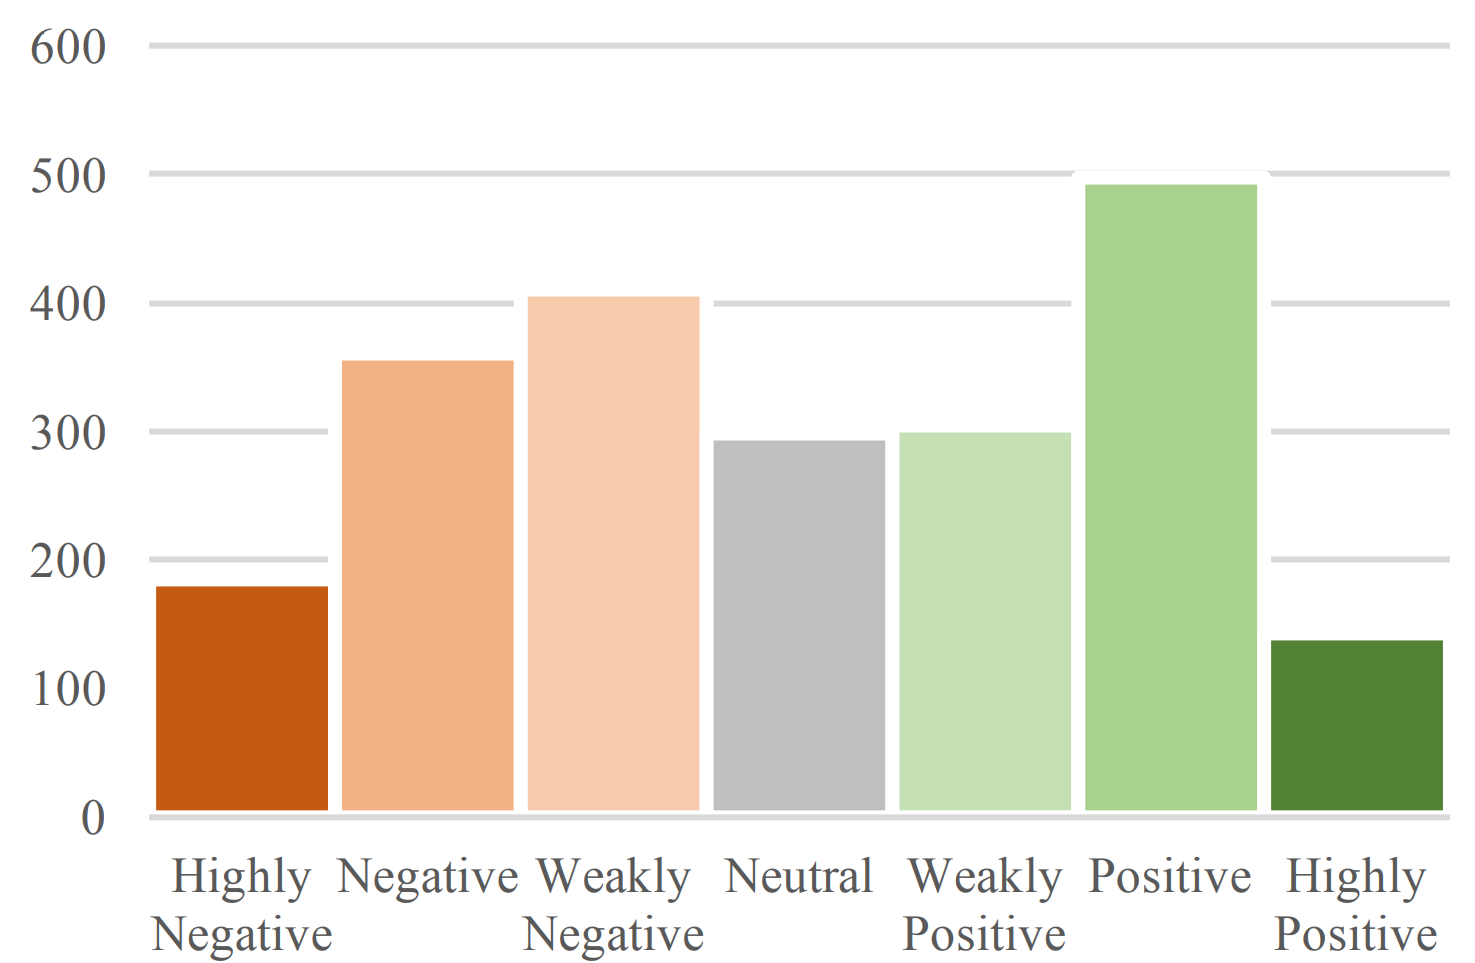
\includegraphics[width=\linewidth]{fig/MOSIhist}
    \caption{Distribution of sentiments over the MOSI dataset, taken from~\cite{zadeh2016mosi}}
    \label{fig:MOSIhist}
\end{figure}

\subsection{MOSEI}
\textit{MOSEI} is the next generation of \textit{MOSI} dataset, a collection of 23453 YouTube video clips from 1000 speakers, with a total time of around 65 hours and 54 minutes. It has the same sentiment labels as \textit{MOSI}, in addition to emotional labels (happiness, sadness, anger, fear, disgust, surprise) labeled by experts. Each video has one speaker and transcribed by its uploader. The distribution of sentiments and emotions over the entire dataset is shown in Figure~\ref{fig:MOSEIhists}. Due to large number of videos contained in this dataset, HPS are needed to process it.

\begin{figure}[t]
	\centering
	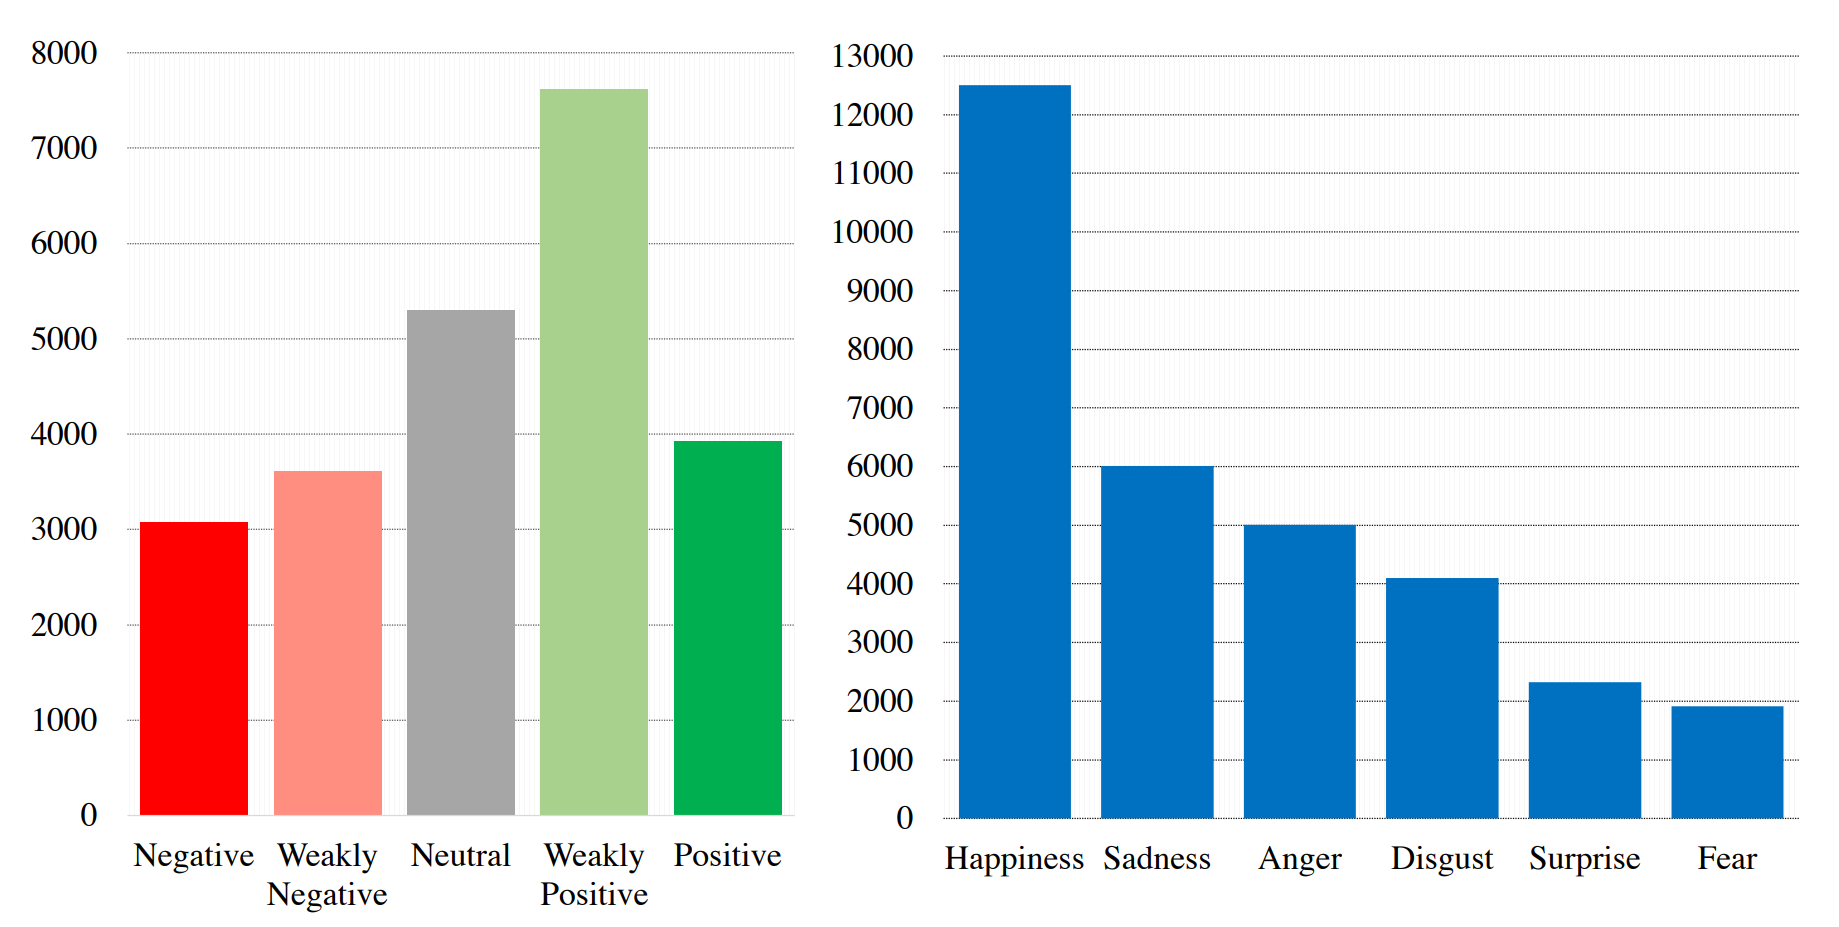
\includegraphics[width=\linewidth]{fig/MOSEIhists}
	\caption{Distribution of sentiments and emotions over the MOSEI dataset, taken from~\cite{zadeh2018multimodal}}
	\label{fig:MOSEIhists}
\end{figure}

\subsection{MSCTD}
Eventually, we decided to use the \textit{MSCTD} dataset. It is a new dataset created in the year 2022 and includes over 17k multi-modal bilingual conversations, consisting of more than 142k English-Chinese and 30k English-German utterance pairs, where each utterance pair corresponds with the associated visual context indicating where it happens. Each visual context of this dataset is a sequence of series or movies images and its dialogues are from OpenViDial dataset~\cite{meng2020openvidial}. In addition, each utterance is annotated with one sentiment label (i.e., positive/neutral/negative). The distribution of sentiments over the entire dataset is shown in Figure~\ref{fig:MSCTDhist}.
\paragraph{} This dataset's annotation includes two steps: automatic annotation and then human annotation, for checking and correcting automatic labeling. The size details of the English-German section of the dataset, which we used in our project, can be seen in table \ref{table:MSCTD}.
\paragraph{} The advantage of this dataset for us was that we wanted to extract numerous features from each scene. In the previous datasets, we mainly had the face of just one speaker, but here we have the complete scene, which allows us to extract additional features, such as different faces, poses, scene details, etc.

\begin{center}
	\begin{table}[h!]
		\begin{tabular}{||c| c c c||} 
			\hline
			Sentiment & Train & Evaluation & Test \\ [0.5ex] 
			\hline\hline
			Positive & 5483 & 1454 & 1606 \\
			\hline
			Neutral & 6921 & 1764 & 1298 \\
			\hline
			Negative & 7836 & 1845 & 2163 \\ [1ex] 
			\hline
		\end{tabular}
	\caption{Number of each utterance in each section in \textit{MSCTD} dataset}
	\label{table:MSCTD}
	\end{table}
\end{center}


\begin{figure}[t]
	\centering
	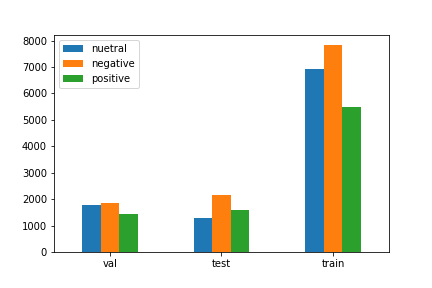
\includegraphics[width=\linewidth]{fig/MSCTDhist}
	\caption{Distribution of sentiments over the MSCTD dataset}
	\label{fig:MSCTDhist}
\end{figure}


\subsection{Other Datasets}
Moreover, there are other datasets that can be used in future works in order to make this project's results more precise. Some of them are:

\begin{enumerate}
	\item \emph{IEMOCAP~\cite{busso2008iemocap}}: Consisted of almost 12 hours of monologues from 10 actors with markers on their faces, heads, and hands, eliciting different emotions during speaking. It needed verification for giving this database which could take a week.
	\item \emph{EmoReact~\cite{nojavanasghari2016emoreact}}: A collected multi-modal basic and complex emotion dataset of children between the ages of four and fourteen years old. It also required up to one-week of verification.
	\item \emph{PATS~\cite{ahuja2020no,ahuja2020style,ginosar2019learning}}: Contains transcribed pose data with aligned audio and transcriptions of 25 speakers of talk shows, lecturers, etc. Using the pose and audio of this dataset can improve our project's outcomes and, therefore, could be considered in future works.
\end{enumerate}

%This section contains some instructions and examples for using \LaTeX.
%
%\subsection{You can add subsections}
%You can use numbered subsections to structure your sections or $\backslash\texttt{paragraph}$ to separate paragraphs with a heading using only a few words, as used in Section~\ref{sec:introduction}.
%
%
%\begin{enumerate}
%	\item\label{item:1} This is an item in an enumeration.
%    \begin{itemize}
%    	\item This is an item of a unnumbered list. In this case, the lists are nested within each other.
%    \end{itemize}
%    \item\label{item:2} The second point in the enumerated list.
%\end{enumerate}
%%
%I can refer to the element of the enumeration above as Point~\ref{item:1}.
%If you refer to numbered items,~e.g. items from a list or figures or sections, always capitalize the name. 
%For example, this is Section~\ref{sec:latex}.
%
%\subsection{Figures}
%You can include figures. You can include files, as done in Figure~\ref{fig:example}. 
%Avoid including jpeg, gif or bmp files since these do not scale nicely. Again Figure~\ref{fig:example} is an example for that.
%
%\begin{figure}[t]
%   \centering
%   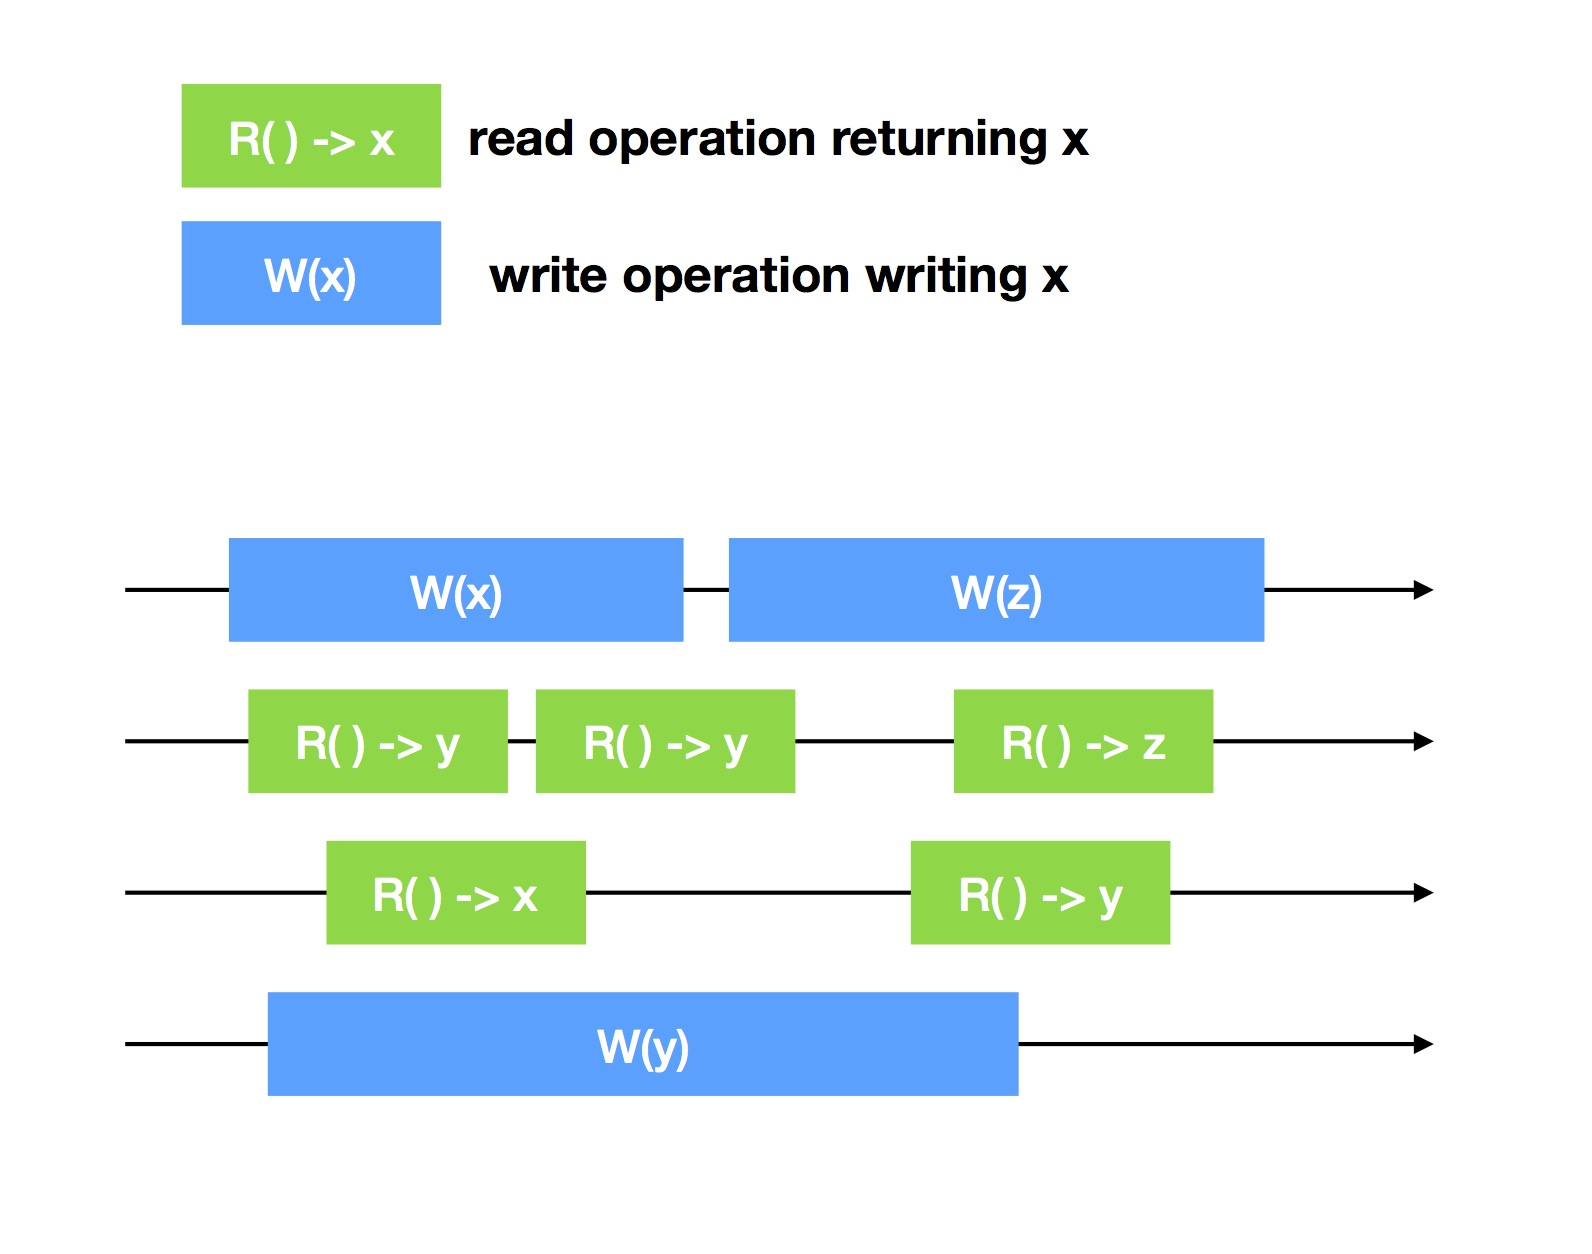
\includegraphics[width=\linewidth]{fig/RegisterOperations}
%    \caption{Figure taken from~\cite{lecture}}
%    \label{fig:example}
%\end{figure}
%
%You can create graphs from your experiment-data using \texttt{pgfplots}.
%See the example in \texttt{tex/evaluation.tex} and documentation \url{http://pgfplots.sourceforge.net/pgfplots.pdf}.
%
%\subsection{Other tips}
%\begin{itemize}
%
%\item Always use the tilde character between the number and unit, e.g. 100~Mbps or 53~ms. The tilde inserts a space, but prevents line break between the number and unit.
%
%\item Never put SI units in italics. 
%
%\item Do differentiate between bits (b) and bytes (B), and between powers of 10~(MB) and 2~(MiB).
%
%\item Avoid things like: "We refer the reader to [42]." That is, don't use citations as nouns.
%\end{itemize}
%
%For further instructions on how to add \textbf{Tables, Algorithms, Theorems see acmguide.pdf}.
